\documentclass[11pt]{beamer}
\usepackage[utf8]{inputenc}
\usepackage[T1]{fontenc}
\usepackage{amsmath}
\usepackage{amsfonts}
\usepackage{amssymb}
\usepackage{graphicx}
\usetheme{default}
\usepackage{subfig}
\begin{document}
	%\author{Carter Rhea}
	\title{Pseudo Arclength Methods in MOOSE}
	%\subtitle{}
	%\logo{}
	%\institute{}
	\date{\today}
	%\subject{}
	%\setbeamercovered{transparent}
	%\setbeamertemplate{navigation symbols}{}
	\frame[plain]{\maketitle}
	
	\begin{frame}
		\frametitle{MOOSE}
		\begin{enumerate}
			\item Multiphysics Object Oriented Simulation Environment
			\item Massively Parallel
			\item Implement Arclength Method in MOOSE
		\end{enumerate}
	\end{frame}

	\begin{frame}
		\frametitle{Pseudo Arclength Method}
		
		\begin{figure}
			\centering
			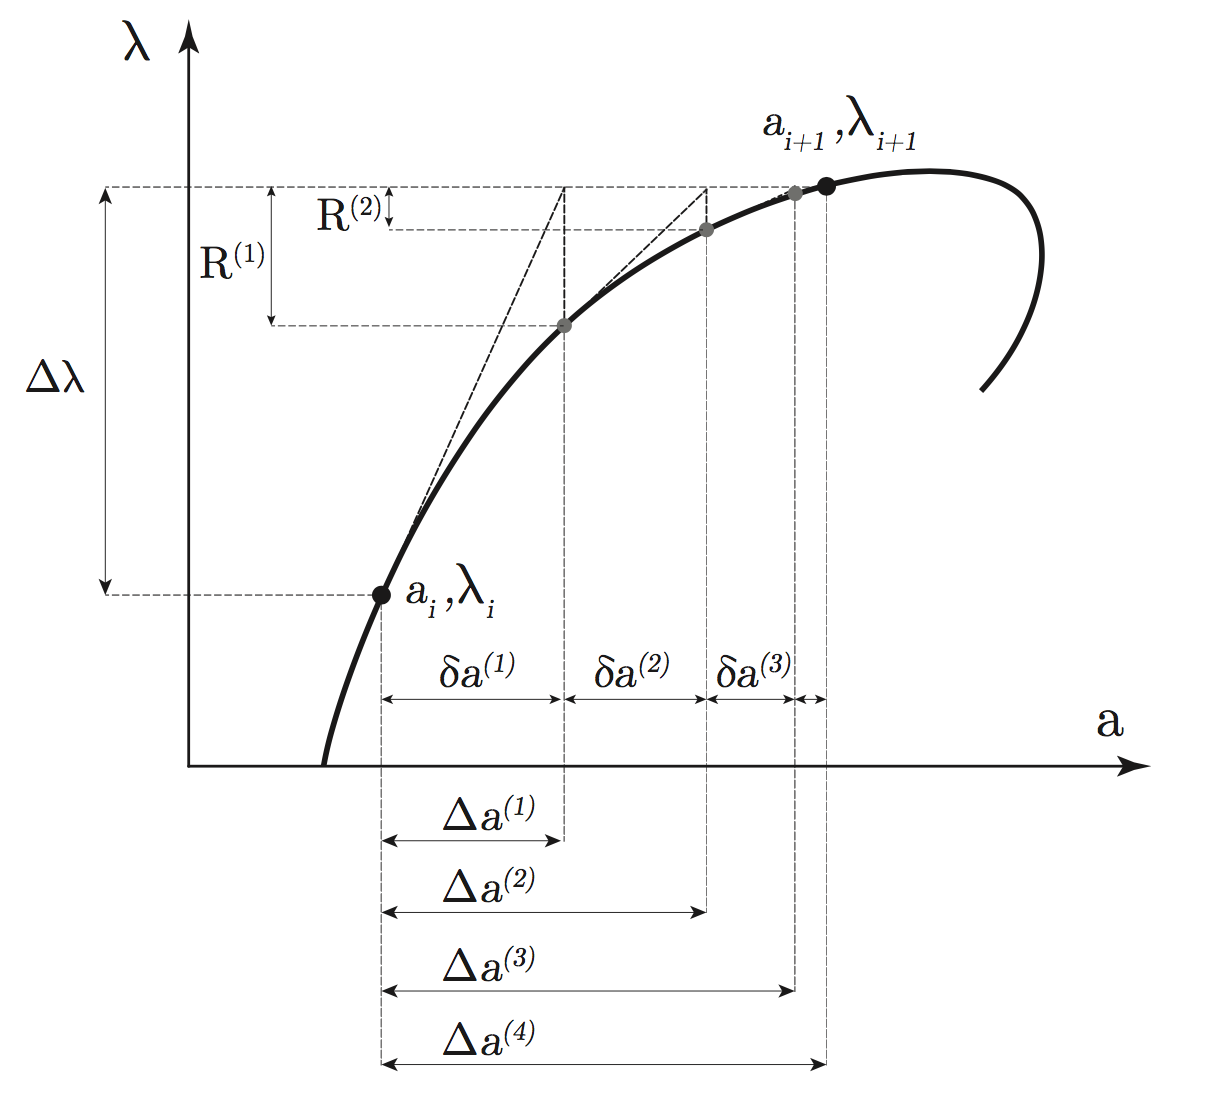
\includegraphics[width=0.5\linewidth]{arclengthschematic}
			\caption{Schematic for Pseudo Arc Length Method \cite{arclength}}
			\label{fig:arclengthschematic}
		\end{figure}
		
	\end{frame}



	\begin{frame}
		\frametitle{Linearized Pseudo Arclength Method}
		$$G(u,\lambda) = (u-u_{old})\frac{\partial u}{\partial s}\Big|_{s_i}+(\lambda-\lambda_{old})\frac{\partial \lambda}{\partial s}\Big|_{s_i} - radius$$	
		Initialization:
		$$\frac{\partial \lambda}{\partial s} \Big|_{s_0} = \frac{1}{\sqrt{2}}$$
		$$\frac{\partial u}{\partial \lambda}\Big|_{s_0} \approx \frac{u_1-u_0}{\lambda_1-\lambda_0} $$ 
		$$\frac{\partial u}{\partial s}\Big|_{s_0} = \frac{\partial \lambda}{\partial s}\Big|_{s_0} \frac{u_1-u_0}{\lambda_1-\lambda_0} $$
		$$\Delta s = \frac{\lambda_1-\lambda_0}{\frac{\partial \lambda}{\partial s}\Big|_{s_0}} $$
		
	\end{frame}

	\begin{frame}
		\frametitle{Results}
		\begin{figure}[!h]
		
			\subfloat[]{\includegraphics[width=0.5\textwidth]{../softening/python/stress_strain}\label{fig:f2}}
				\subfloat[]{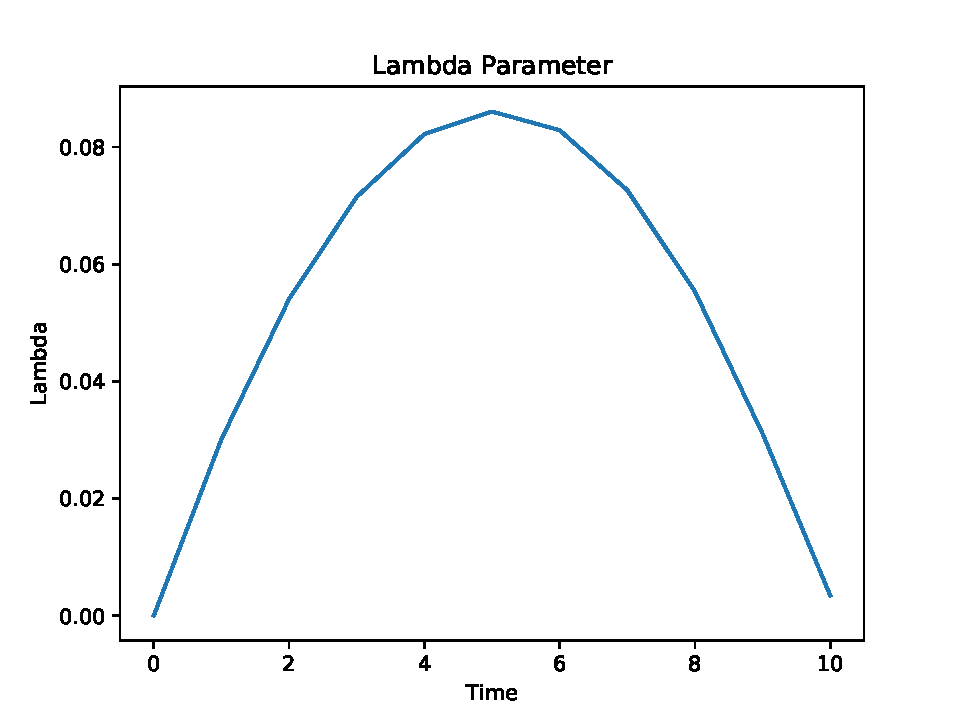
\includegraphics[width=0.5\textwidth]{lambda_CL}\label{fig:f1}}
		
			
		\end{figure}
	\end{frame}

	\begin{frame}
		\frametitle{Coupling Damage with Phase Field}
		
\begin{figure}
\centering
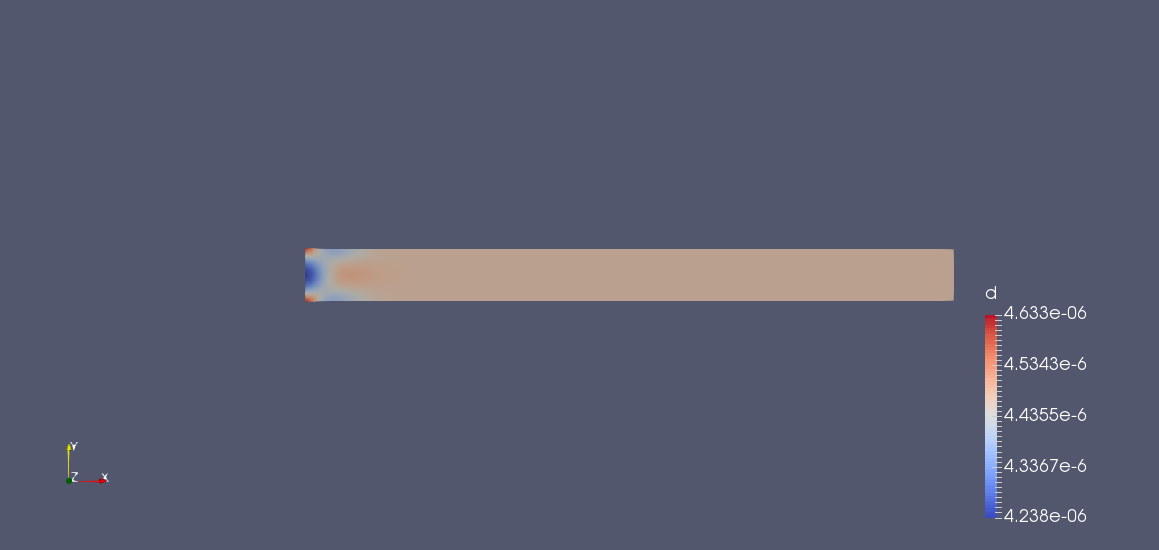
\includegraphics[width=0.7\linewidth]{tension_basic}
\caption{Bar under tension with dirichlet BC on left. No softening.}
\label{fig:tension_basic}
\end{figure}
	\end{frame}
	
	
	
	
	
	
	
	
	
	\begin{frame}
			\begin{thebibliography}{9}
				\bibitem{arclength} 
				A. G. Salinger, N. M. Bou-Rabee, R. P. Pawlowski, E. D. Wilkes, E. A.
				Burroughs, R. B. Lehoucq, and L. A. Romero. Sand2002-0396: Loca 1.0
				library of continuation algorithms: Theory and implementation manual.
				Technical report, Sandia National Laboratories, Albuquerque, NM, 2002.
				\bibitem{moose}https://github.com/idaholab/moose
			\end{thebibliography}
	\end{frame}



\end{document}